% % % % % % % % % % % % % % % % % % % % % % % % % % % % % % % % % % % % % % % % % % % %
%                                                                                     %
% Short Sectioned Assignment LaTeX Template Version 1.0 (5/5/12)                      %
% This template has been downloaded from: http://www.LaTeXTemplates.com               %
%                                                                                     %
% Original author:  Frits Wenneker (http://www.howtotex.com)                          %
%                                                                                     %
% Modified by: Fco Javier Sueza Rodríguez (fcosueza@disroot.org)                      %
%                                                                                     %
% Changes:                                                                            %
%	    - Custom Chapters, Sections and Subsections (titlesec package)                %
%           - Document type scrbook (oneside)                                         %
%           - Use babel-lang-spanish package and marvosym                             %
%           - Use hyperref, enumitem, tcolorbox and glossaries packages               %
%           - Use Time New Roman (mathptmx), Helvetic and Courier fonts               %
%                                                                                     %
% License: CC BY-NC-SA 3.0 (http://creativecommons.org/licenses/by-nc-sa/3.0/)        %
%                                                                                     %
% % % % % % % % % % % % % % % % % % % % % % % % % % % % % % % % % % % % % % % % % % % %

%-----------------------------------------------%
%	              Packages                  %
%-----------------------------------------------%

\documentclass[paper=a4, fontsize=11pt, oneside]{scrbook}

% ---- Text Input/Output ----- %

\usepackage[T1]{fontenc}
\usepackage[utf8]{inputenc}
\usepackage{mathptmx}
\usepackage[scaled=.92]{helvet}
\usepackage{courier}
\usepackage[indent=12pt]{parskip}

\usepackage{geometry}
\geometry{verbose,tmargin=3cm,bmargin=3cm,lmargin=2.6cm,rmargin=2.6cm}

% ---- Language ----- %

\usepackage[spanish]{babel}
\usepackage{marvosym}

% ---- Another packages ---- %

\usepackage{amsmath,amsfonts,amsthm}
\usepackage{graphics,graphicx}
\usepackage{titlesec}
\usepackage{fancyhdr}
\usepackage{tcolorbox}
\usepackage{hyperref}
\usepackage{enumitem}
\usepackage[automake]{glossaries}

%--------------------------------------------------------------------%
%                      Customizing Document                          %
%--------------------------------------------------------------------%


% ----------- Custom Chapters, Sections and Subsections -------------- %

\titleformat{\chapter}[display]
			{\bfseries\Huge}
			{Tema \ \thechapter} {0.5ex}
			{\vspace{1ex}\centering}

\titleformat{\section}[hang]
			{\bfseries\Large}
			{\thesection}{0.5em}{}

\titleformat{\subsection}[hang]
			{\bfseries\large}
			{\thesubsection}{0.5em}{}

\titleformat{\subsubsection}[hang]
			{\bfseries\large}
			{\thesubsubsection}{0.5em}{}

\hypersetup{
    colorlinks=true,
    linkcolor=black,
    urlcolor=magenta
}

% ------------------- Custom heaaders and footers ------------------- %

\pagestyle{fancyplain}

\fancyhead[]{}
\fancyfoot[L]{}
\fancyfoot[C]{}
\fancyfoot[R]{\thepage}

\renewcommand{\headrulewidth}{0pt} % Remove header underlines
\renewcommand{\footrulewidth}{0pt} % Remove footer underlines

\setlength{\headheight}{13.6pt} % Customize the height of the header

% --------- Numbering equations, figures and tables ----------------- %

\numberwithin{equation}{section} % Number equations within sections
\numberwithin{figure}{section} % Number figures within sections
\numberwithin{table}{section} % Number tables within sections

% ------------------------ New Commands ----------------------------- %

\newcommand{\horrule}[1]{\rule{\linewidth}{#1}} % Create horizontal rule command


%----------------------------------------------------------------------------------------
%	TÍTULO Y DATOS DEL ALUMNO
%----------------------------------------------------------------------------------------

\title{
\vspace{10ex}
\normalfont \normalsize
\Huge  \textbf{SITE WISE}
}
\author{Francisco Javier Sueza Rodríguez}

%----------------------------------------------------------------------------------------
%                                     DOCUMENTO
%----------------------------------------------------------------------------------------
\begin{document}

\maketitle

\thispagestyle{empty}


\vspace{73ex}

\begin{center}
    \begin{tabular}{l l}
        \textbf{Centro}: & IES Aguadulce \\
        \textbf{Ciclo Formativo}: & Desarrollo Aplicaciones Web (Distancia)\\
        \textbf{Asignatura}: & Empresa e Iniciativa Emprendedora\\
        \textbf{Tema}: & Tema 6 - El plan de inversiones y el plan financiero\\
    \end{tabular}
\end{center}

\newpage

\tableofcontents

\newpage

\section{Resumen Ejecutivo}


\section{La Idea de Negocio}
El proyecto que se va a presentar hoy es \textbf{Site Wise}, una empresa de desarrollo web especializada en asesoramiento, creación de páginas web y presencia online para PyMES y grandes empresas. Hoy en día la \textbf{presencia en internet} es vital para cualquier negocio, ya sea grande o pequeño, y la implementación de tiendas online pueden suponer un gran incremento en la visibilidad y la venta de cualquier empresa.

En \textbf{Site Wise} nos encargamos de buscar la mejor solución a las necesidades de nuestros clientes. Por un lado, ofrecemos servicios para le creación de páginas web económicas, utilizando herramientas como \textbf{Wordpress} para que las \textbf{pequeñas empresas} que no cuentan con presupuestos elevamos puedan poner su negocio en la web, o montar una tienda online de forma rápida y asequible. Por otro lado, ofrecemos \textbf{web más personalizadas}, de más alto coste, para empresas con mayor presupuesto y que demandan la realización de aplicaciones web con tecnologías específicas.

Además, estos dos servicios se complementan con un \textbf{servicio de asesoramiento}, para guiar al cliente en la puesta en internet de su negocio así como de un \textbf{servicio de mantenimiento} que asegura que se puedan realizar cambios en la web, requeridos por el cliente, a un bajo coste.

\begin{figure}[H]
    \centering
    
\includegraphics[scale=0.40]{logo-empresa.png}
    \caption{Logotipo de la Empresa}
\end{figure}

\section{Responsabilidad Social y Cultura de Empresa}
Las principios de la empresa son dar una \textbf{trato cercano a los clientes}, adaptando el desarrollo a sus necesidades y a sus posibilidades económicas. Los equipos y el \textbf{consumo energético} debe ser responsable con el medio ambiente, primando compañías para el suministro que empleen fuentes de \textbf{energía renovables}, intentado minimizar la huella de carbono generada por la empresa.

En \textbf{futuras ampliaciones de plantilla}, se optaría por una \textbf{organización plana} donde todos los empleados cuentan, primando su \textbf{bienestar laboral}, la \textbf{conciliación familiar} y el \textbf{desarrollo profesional} de estos, creando un ambiente de trabajo lo más agradable posibles para los empleados.

\section{Promotores}
El promotor del proyecto es \textbf{Francisco Sueza} (es decir yo), soy una persona dinámica con buena capacidad analítica a la que le gusta la resolución de problemas, analizando las diferentes soluciones y aplicando la más adecuada a la situación. Soy una persona creativa, proactiva y empática a la que le encantan los desafíos y que no escatima tiempo ni esfuerzo a la hora de cumplir las metas que me propongo, utilizando para ello las herramientas adecuadas.

\subsection{Datos Personales}

\begin{itemize}
    \item \textbf{Nombre y Apellidos}: Francisco Javier Sueza Rodríguez
    \item \textbf{Dirección}: Calle Arrayanes, n6, 4º A
    \item \textbf{Teléfono}: 640585461
    \item \textbf{Correo}: fcosueza@gmail.com
    \item \textbf{Formación Relacionada}:
    \begin{itemize}
        \item \textbf{2004}: Curso FPO “Programación de Aplicaciones Informáticas” en Centro de Estudios Hnos.
        Naranjo, Granada (950h).
        \item \textbf{2020}: Certificado “Diseño Web Responsive” en freeCodeCamp (300h)
        \item \textbf{2021}: Certificado “Algoritmos y estructuras de datos en Javascript” en freeCodeCamp (300h)
        \item \textbf{2022 - Actualidad}: Grado Superior de Desarrollo de Aplicaciones Web (IES Aguadulce)
    \end{itemize}
    \item \textbf{Experiencia Laboral Relacionada}:
    \begin{itemize}
        \item \textbf{2022 - Actualidad}: Desarrollador Web Freelance, desarrollando páginas web, utilizando diferentes herramientas, desde su concepción hasta su puesta en marcha.
    \end{itemize}
    \item \textbf{Habilidades Relacionadas con el Proyecto}:
    \begin{itemize}
        \item \textbf{Diseño de Interfaces}: diseño de interfaces siguiendo los estándares de accesibilidad y buenas prácticas para la experiencia de usuario.
        \item \textbf{Lenguajes de Programación}: Javascript, Java, Ruby, C++, HTML, CSS.
        \item \textbf{Librerias y FrameWorks}: React, Node, SASS, testing library, Jest.
        \item \textbf{Diseño}: Figma, Diseño Responsivo, UX.
    \end{itemize}
    \item \textbf{Motivación}: el desarrollo web es mi pasión, y estoy entusiasmado por la creación de productos de calidad. Siendo mi propio jefe puedo establecer la ruta de la empresa estableciendo buenos estándares de calidad y un proceso de desarrollo innovador para aportar nuevas ideas al sector.
\end{itemize}

\section{Análisis del Entorno}
En este apartado vamos a realizar una análisis del entorno tanto general como especifico de la empresa, que podemos ver de forma detallada en los siguientes subapartados.

\subsection{Entorno General}
En este epígrafe analizamos el entorno general que rodea a nuestro proyecto, y como es de propicio para el desarrollo de nuestra idea.

\subsubsection{Factores Económicos}
Actualmente hay una situación financiera relativamente estable, con una creación de empleo sostenida en el tiempo, aunque las tasas de paro aún siguen siendo elevadas. Se han realizado varias subidas del SMI aunque esta ganancia de poder adquisitivo se ha visto mermada por la gran inflación a la que esta sometido el país y la zona euro en los últimos años. Esta inflación elevada, por suerte, no afecta tanto al sector del desarrollo de software, en cambio si esta afectando al poder adquisitivo de la población. A pesar de ello, el PIB del país sigue creciendo aunque a un ritmo más lento.

\subsubsection{Factores Socioculturales}
En España tenemos una sociedad que aunque esta envejeciendo, debido a la baja natalidad y la alta esperanza de vida, hace un uso intensivo de las nuevas tecnologías especialmente en las generaciones más jóvenes, las cuales valoran mucho el tiempo libre y de ocio, muchas veces ligado a estas nuevas tecnologías. Hay un nivel cultural relativamente alto y el estado proporciona ayudas y servicios para asegurar el estado de bienestar, si bien en los últimos años ha habido una degradación en los servicios sanitarios que se ha visto acentuada por el paso de la Pandemia del COVID.

En general, es una sociedad bastante digitalizada, con un 70\% de la población con competencias básicas en nuevas tecnologías y un indice de alfabetización del 98\%.

\subsubsection{Factores Políticos}
Actualmente España tiene un gobierno progresista integrado por varios partidos políticos siendo el principal el PSOE. La estabilidad política es relativa, ya que actualmente depende de los pactos con partidos regionalistas y no esta asegurada la aprobación prácticamente de ninguna ley por adelantado, por lo que tienen que estar negociando continuamente para la aprobación de dichas leyes.

En el aspecto internacional, España esta integrado en la Unión Europea y el Espacio Económico Europeo, por lo que los trabajadores y ciudadanos en general tienen libre circulación por los países de la UE. Además hay menos trabas para desarrollar la actividad económica en estos países, siendo de aplicación también la normativa europea en territorio español respecto a las empresas y el desarrollo de actividades económicas.

\subsubsection{Factores Legales}
España tiene una fuerte legislación respecto a las relaciones laborales y la creación de empresas, cuya base es el Estatuto de los Trabajadores, que garantiza los derechos fundamentales de los trabajadores y establece un marco para las relaciones laborales.

Además del Estatuto de los Trabajadores tenemos los Convenios Colectivos que son de aplicación a sectores específicos y regulan la actividad la laboral en estos sectores, usando como marco el Estatuto de los Trabajadores, ampliando según las necesidades de cada sector los derechos y deberes recogidos en éste.

Hay instaurado un sistema de Seguridad Social, un sistema de seguro de salud que garantiza a la población contra los costes de la asistencia sanitaria, así como es establecimiento de un sistema de pensiones por jubilación, invalidez, etc. El sistema se sustenta con las aportaciones de trabajadores y empresarios, siendo un sistema contributivo.

Cabe también destacar la políticas de protección de datos aplicables y que afectan especialmente al sector de las nuevas tecnologías, habiendo leyes tanto estatales, así como la Agencia Española de Protección de Datos, como son también de aplicación las leyes europeas en este asunto, siendo una de las leyes más restrictivas que hay ahora mismo en el mundo, siendo el Reglamento General de Protección de Datos (RGPD) la principal ley de aplicación en la UE.

\subsubsection{Factores Tecnológicos}
Hoy en día la tecnología esta presenten en todos los ámbitos de la vida. En España hay un alto grado de digitalización tanto en el entorno empresaria como en el de la administración pública.

Las TIC están revolucionando el mundo empresarial, desde aspectos como el marketing y la búsqueda de clientes, como la automatización de los procesos empresariales y la interacción de las empresas con el entorno. En este aspecto, las aplicaciones web ofrecen un escaparate que incrementa la visibilidad de la empresas permitiéndoles presentar sus productos a más clientes en diferentes países y que permitiendo que se puedan hacer transacciones de forma rápida y segura.

La amplia utilización de internet y la web hace que sea el medio ideal para que las empresas se den a conocer a ellas mismas y sus productos, así como a promocionar los valores que fomentan. Además, con el auge del e-commerce la presencia en internet y la venta de productos por este medio se esta convirtiendo en algo indispensable, si se quieren aumentar las ventas de una empresa.

\subsubsection{Factores del Sector}
El sector del desarrollo de software es un sector que esta actualmente en auge en España y la mayoría de países industrializados, ya que el nivel de alta digitalización de estos países y el uso masivo de internet y las TIC ha creado la necesidad de software especializado y la creación de aplicaciones web.

En la actualidad, hay muchas empresas de de desarrollo de software. Son empresas que se caracterizan por buenas condiciones de trabajo, con salarios por encima de la media y con especial énfasis en el bienestar del trabajado y la conciliación laboral.

Es un sector en el que el teletrabajo esta ganando cada vez más terreno y las bonificaciones, como seguros privados, equipos informáticos proporcionados por la empresa, etc.., están a la orden del día.

En este aspecto, hay que ofrecer condiciones de trabajo que sean atractivas para poder mantener el talento, ya que con la gran cantidad de empresas y la alta demanda de profesionales, sin unas buenas condiciones los profesionales acabarán cambiando de compañía, y es crucial tener profesionales con gran talento para crear productos software de calidad y de una forma eficiente.

\subsection{Entorno Específico}
Ahora, pasamos a analizar el entorno específico de nuestro proyecto, analizando la competencia que nos podemos encontrar así como los posibles clientes entre otras cosas.

\subsubsection{Competencia}
En Granada hay un buen número de empresas de desarrollo de software y desarrollo web. Caben destacar algunos grupos grandes como Nazaríes, que es una consultora que ha adquirido ademas algunas empresas de desarrollo web.

El problema con muchas de las empresas en Granada es que los sueldos son muy bajos en comparación a la media del sector en el resto del país por lo que tienen dificultades para retener talento.

Nuestra ventaja es que vamos a cambiar esto, ofreciendo sueldos y condiciones más competitivos para retener programadores con talento lo que nos va a dar una ventaja en la calidad del producto y en los costes de producción.

\subsubsection{Clientes}
Nuestros clientes van a estar situados en dos segmentos muy concretos. Por un lado estarán las PyMES y por otro lado las grandes empresas.

\textbf{PyMES}: en las PyMES vamos a encontrar clientes con una poder adquisitivo variable, desde bajo hasta alta, aunque este tipo de clientes van a demandar webs a unos precios más asequibles. Tampoco vamos a encontrar muchos clientes con conocimientos técnicos sobre desarrollo web y probablemente necesitarán más asesoramiento sobre como enfocar la puesta de su negocio en internet.

\textbf{Grandes Empresa}s: en este segmento vamos a encontrar clientes con gran poder adquisitivo y probablemente con una idea muy clara de que tipo de aplicación web quieren. Podrán más énfasis en la calidad del producto y van a necesitar menos asesoramiento sobre el proceso de puesta en marcha de la web y del negocio en la red.

\subsubsection{Proveedores}
Dada la naturaleza de la actividad de la empresa no se van a necesitar intermediarios, si formamos un equipo multidisciplinar que cubra todas las necesidades del proceso de desarrollo web.

Los proveedores van a ser limitados. En concreto nuestro proveedor de suministro eléctrico va a ser PepeEnergy, que proporciona energía 100% renovable acorde a nuestros ideales de mínimo impacto en el medio ambiente.

Respecto a los equipos informáticos. Se diseñaran específicamente los servidores necesarios y los equipos que se deban montar para los programadores, diseñadoras y administradores de redes. Estos equipos serán adquiridos a través de Amazon, ya que proporciona unas garantías y facilidades para de devolución, cambio y reparación que no ofrecen otros proveedores y que pueden agilizar este tipo de procesos.

Así mismo, el material propio de oficina será adquirido a través de esta plataforma, por las mismos motivos que ya hemos comentado.

\subsubsection{Presciptores}
Las principales personas que van a recomendar nuestros servicios son los propios clientes, por lo que debemos asegurar que quedan satisfechos y que se les da un buen soporte a las aplicaciones que desarrollemos.

\section{Análisis DAFO}
Nuestra idea, como cualquier proyecto, tiene sus puntos fuertes y sus puntos débiles, así como un conjunto de oportunidades que tenemos que aprovechar sin dejar de prestar atención a las amenazas. A continuación, listamos todos estos puntos.

\begin{itemize}
    \item \textbf{Debilidades}:
    \begin{itemize}
        \item Falta de experiencia
        \item Red de contactos mejorable
        \item Pocos recursos económicos
        \item Empresa emergente que puede resultar poco atractiva para programadores experimentados
    \end{itemize}

    \item \textbf{Amenazas}:
    \begin{itemize}
        \item La alta inflación ha mermado el poder adquisitivo de los posibles clientes, especialmente a nivel local.
        \item Empresas mas grandes que pueda ofrecer productos a precios más económicos..
        \item Las adquisición inicial de programadores con talento es complicada, debido a la  alta demanda de profesionales que hay en el sector.
        \item A nivel local, aún hay muchas pequeñas empresas que no muestran interés por las TIC debido al desconocimiento de las ventajas que ofrecen.
    \end{itemize}

    \item \textbf{Fortalezas}:
    \begin{itemize}
        \item Inversión inicial pequeña en comparación con otro tipo de empresas.
        \item Costes de producción bajos
        \item Productos de calidad a precios competitivos
        \item Uso de tecnologías punteras que no se emplean en la mayoría de empresas locales
    \end{itemize}

    \item \textbf{Oportunidades}:
    \begin{itemize}
        \item Sector de las TIC en pleno crecimiento y con una alta demanda de aplicaciones web en el sector 	empresarial, especialmente a nivel estatal e internacional.
        \item Posibilidad de contacto con clientes de cualquier parte de España y Europa.
        \item Posibles ayudas estatales para el emprendimiento y la innovación.
        \item Auge del e-commerce que esta creando una gran demanda de tiendas digitales para todo tipo de empresas.
    \end{itemize}
\end{itemize}

\section{Plan de Marketing}
Nuestro plan de marketing se cimienta en el trato a los clientes y la elaboración de productos software de calidad, como señas de identidad.

\subsection{Nuestros Clientes}
Las PyMES, en su mayoría serán clientes a nivel local o estatal, con un poder adquisitivo variable y con conocimientos bajos o medios sobre las TIC.

Estos clientes necesitarán asesoramiento extra para concretar la características de la aplicación web a desarrollar analizando sus necesidades y proponiendo diferentes soluciones que se puedan adaptar a estas. Aunque no tengan conocimientos altos sobre TIC, si harán uso de estas en su vida cotidiana por lo que serán conscientes de la relevancia a nivel social que tienen éstas.

Por otro lado tenemos las Grandes Empresas. Este segmento se caracteriza por clientes que tienen muy claro las necesidades que tienen y que piden productos muy específicos con pocas necesidades de asesoramiento. Son clientes de alto poder adquisitivo y probablemente con presencia internacional. Clientes por norma general con mayor nivel de formación y con exigencias de calidad mayores que las que nos podemos encontrar en las PyME.

\subsection{Marcando la Diferencia}
Nuestra principal ventaja va a ser la calidad de los productos que vamos a ofrecer. Estableciendo un proceso de desarrollo que nos permite verificar la calidad del producto en cada etapa y pudiendo realizar entregas de forma ágil y presentar la evolución del producto a cliente de forma continua y rápida.

Además, hay dar un trato personal y cercano especialmente a las PyMES, ya que suelen ser negocios pequeños, en muchas ocasiones incluso familiares y que no están tan familiarizados con las TIC a nivel empresarial como las Grandes Empresas o las Starups, porque lo que un trato cercado y realizar una labor pedagógica sobre las ventajas de las TIC es crucial con estás empresas.

\subsection{Política de Producto}
Nuestros productos están pensados para adaptarse a las necesidades de nuestros clientes, pensando en sus necesidades económicas, y en las diferentes características que tienen nuestros clientes.


\subsubsection{Productos}


\begin{itemize}
    \item \textbf{Wordpresss y E-Commerce}

    Para los presupuestos más ajustados ofrecemos desarrollo con Wordpress y Magento, que permitirán a tu negocio darse a conocer en la web y poder vender tus productos de forma rápida y eficiente.

    \textbf{Precio}: 1000€ - 5000€

    \item \textbf{Asesoramiento TIC}

    Con este servicio se ofrece asesoramiento sobre TIC para orientar a nuestros clientes sobre las posibilidades que ofrecen las TIC para su negocio y las ventajas que puede ofrecer su uso.

    \textbf{Precio}: 30€/h

    \item \textbf{Aplicaciones Web}

    Si tienes claro lo que quieres, nuestro servicio de desarrollo de aplicaciones usa las últimas tecnologías en desarrollo web para crear aplicaciones de calidad y eficientes para tu empresa.

    \textbf{Precio}: 5000€ en adelante

    \item \textbf{Servicio de Mantenimiento}

    Con este servicio se le ofrece al cliente la posibilidad de pagar una cuota mensual que cubrirá la solución de posibles errores en los productos contratados y que surjan como consecuencia de su uso así como pequeñas modificaciones en éstos.

    \textbf{Precio}: 50€/mes (Wordpress) y 200€/mes (Aplicaciones Web).

\end{itemize}


\subsubsection{Calculo de los Precios}
El cálculo de los precios exacto es complicado, ya que este va depender en gran medida de la complejidad de la aplicación que se vaya a desarrllora, por eso, en productos como el desarrollo con \textbf{Wordpress} y las \textbf{Aplicaciones Web} se ha establecido un arco de precios aproximado.

En el caso de del \textbf{asesoramiento TIC}, del cual me encargaré personalmente, se ha establecido un precio de 30€/h. En el servicio de mantenimiento de ha establecido 2 precios dependiendo del producto que se haya contratado, ya que la complejidad de solucionar errores o realizar pequeñas modificaciones varia mucho entre un producto y otro. Por ellos se ha establecido un cuota de 50€/mes para los productos con Wordpress y de 200€/mess para las aplicaciones web.

Para los desarrollos, tanto de Wordpress como de Aplicaciones Web, se han tenido en cuenta los \textbf{costes de producción}, calculando cuanto será el coste de una \textbf{hora de trabajo} teniendo en cuenta los empleados que se dedicarán a ello. Se ha excluido mi salario, ya que este se incluye dentro de los beneficios de la empresa.

Se ha tenido en cuenta que a parte del promotor, que cumplirá funciones de product manager y desarrollador, se necesitará un \textbf{diseñador web}, que se encargará de realizar el diseño de las páginas web así como de los desarrollos en Wordpress y E-commerce. Además, se necesitará otro \textbf{desarrollador web}, para poder manejar varios proyectos al mismo tiempo y un administrador de redes, que se encargará de establecer, configurar y administrar la red de la empresa. Se ha estimado que la hora de trabajo de cada trabajador tendrá un coste de \textbf{40€/h}, por lo que se ha calculado, teniendo en cuenta que habrá 2 trabajadores dedicado en exclusiva a los proyectos de Wordpress, y que estos desarrollos tendrán un coste de \textbf{140€/h}, y los desarrollos web, donde habrá 3 trabajadores implicados un coste de \textbf{200€/h}.

Descontando los gatos, estimados en 20€/h, da un beneficio de 40€/h por proyecto de Wordpress y de  60€/h en desarrollos web. Esto supone un \textbf{beneficio bruto del 30\%} sobre los proyectos desarrollados.


\subsection{Política de Comunicación}
\label{sec:publi}
El principal canal de comunicación será internet, pero si queremos también captar negocios locales debemos explorar otros canales que lleguen también a negocios más tradicionales. Por ello se han establecido las siguientes políticas de comunicación:

\begin{enumerate}
    \item En primer lugar se creará una campaña de \textbf{google ads} que se mantendrá en el tiempo, incluyendo anuncios en Youtube. El coste estimado de este servicio será de unos 500€/mes, aproximadamente.
    \item También se establecerá un anuncio en el \textbf{periódico local}. Se han elegido los Domingos alternos, como día para que se muestra el anuncio, que aunque su coste es más elevado, es el día de la semana donde más periódicos se venden. El coste estimado este servicios es de unos 200€/mes.
    \item Por último, cada 3 meses durante los primeros 2 años, se realizará la \textbf{impresión de tarjetas de presentación} y se realizará su distribución en los negocios locales, con un coste estimado de 500€/año.
\end{enumerate}

El coste estimado total será de \textbf{ 8.900€/año}.

\section{Localización}
La localización en el caso de este proyecto no es una factor determinante, ya que los clientes se captaran principalmente de forma telemática y el trabajo se realizará en una oficina.

Dadas estas circunstancias, se ha elegido un pueblo de la periferia de Granada, en concreto \textbf{Armilla}, que se encuentra a 10 min. En concreto la oficina se encuentra en  \textbf{Calle de Lérida, 3, Armilla, Granada}, es una zona residencial y el edificio cuenta con varias oficinas. La ubicación cuenta con \textbf{todos los servicios básicos} y además tiene una \textbf{parada de metro} cercana.

La oficina ya cuenta con \textbf{material básico} como \textbf{escritorios}, \textbf{aires acondicionados}, \textbf{estanterías},... por lo que esto supondrá menos gasto inicial. Tiene una superficie de \textbf{90m2} y el precio de alquiler es de \textbf{450€/mes}, donde están incluidos los servicios de \textbf{luz}, a\textbf{agua} e \textbf{internet}.

Por todo esto, esta oficina es una inmejorable opción, ya no solo porque el gasto mensual es bajo, teniendo en cuenta los servicios que se incluyen en el precio, sino porque esta en un ambiente inmejorable de tranquilidad para el desarrollo de la actividad, teniendo además una buena terraza con vistas a la sierra donde se colocarán sillas y mesas para que los trabajadoras se puedan relajar.

A continuación se muestra una imagen de la oficina, tal y como aparece en la plataforma de alquiler.

\begin{figure}[H]
    \centering
    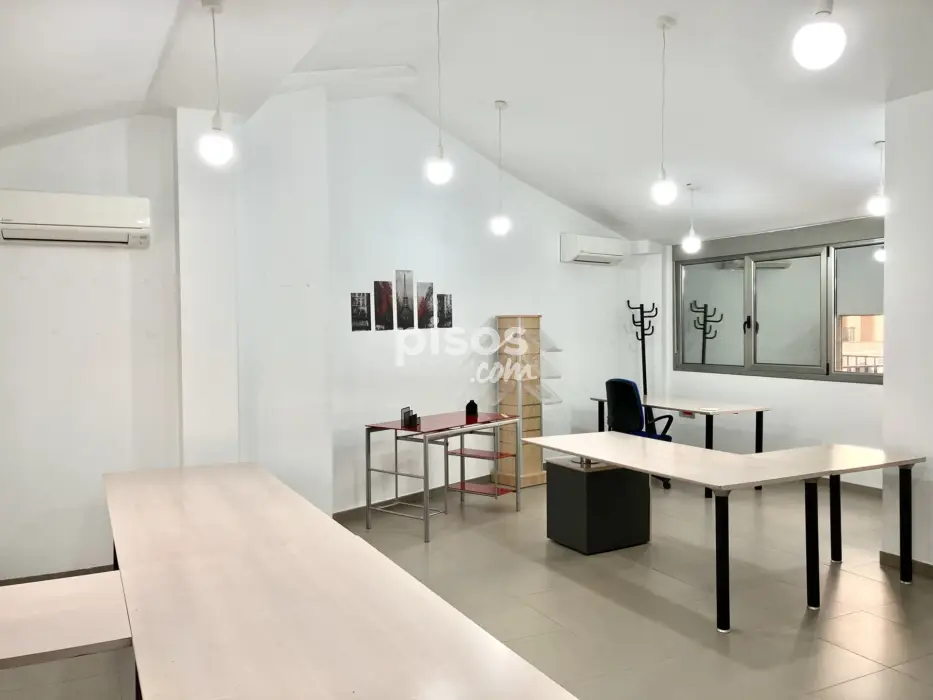
\includegraphics[scale=0.30]{oficina.png}
    \caption{Oficina elegida para el proyecto}
\end{figure}

\section{Plan de Operaciones}
En este apartado se va a detallar el plan de operaciones, especificando, con diferentes apartados donde especificaremos cada uno de los detalles del plan que afectan para el correcto funcionamiento de la empresa.

\subsection{Gestión del Aprovisionamiento}
Debido a la naturaleza de la empresa, no hay que realizar una gestión de aprovisionamiento muy complejo. Durante el proceso de puesta en marcha de la empresa se adquirirán los materiales y dispositivos necesarios para el desarrollo de software, siendo solo necesario la reposición de material de oficina de forma mensual.

El \textbf{material inicial} que se necesitará entra dentro de dos categorías, el \textbf{material de oficina} y los \textbf{dispositivos informáticos}. Para el correcto funcionamiento de la empresa necesitaremos los siguientes elementos:

\begin{itemize}
    \item \textbf{Material de Oficina y mobiliario}: dentro de esta categoría podemos encontrar los siguientes elementos:
    \begin{itemize}
        \item \textbf{Escritorios} para todos los puestos (4 escritorios)
        \item \textbf{Sillas ergonómicas} de calidad para todos los puestos y una para el despacho (5 sillas ergonómicas)
        \item \textbf{Pizarra blanca} de gran tamaño para realizar esquemas y anotaciones (1 pizarra).
        \item \textbf{Lapiceros}, \textbf{folios}, \textbf{bolígrafos}, etc., que deberán estar en cada puestos.
        \item \textbf{Papeleras} repartidas por al oficina (3 papeleras).
        \item \textbf{Sofás} y \textbf{mesas} para la zona de esparcimiento y descanso (2 sofás y 1 mesa).
        \item \textbf{Jabón de manos}, \textbf{papel higiénico} y elementos de aseo para el lavabo.
    \end{itemize}

    \item \textbf{Dispositivos y Equipos informáticos}: en este categoría entran todos los ordenadores y servidores que necesitará la empresa. Así tenemos:

    \begin{itemize}
        \item \textbf{Ordenadores de Sobremesa o Portátiles}: se necesitarán ordenadores para cada puesto, además de un servidor para ofrecer diferentes servicios durante el proceso de desarrollo. Preferiblemente serán ordenadores portátiles, aunque dentro de un
        presupuesto establecido se le ofrecerá a cada desarrollador que elija un PC o portátil de su elección (3 PCs o Portátiles)

        \item \textbf{Servidor}: un servidor será necesario para el desarrollo eficiente de la actividad. No es necesario que sea un servidor de altas prestaciones ya que la empresa es pequeña y somos pocos trabajadores, por lo que se podrá ajustar el presupuesto. (1 servidor)

        \item \textbf{Elementos de red}: además se necesitará algunos elementos de red, en concreto un hub y un número determinado de metros de cable UTP para montar la red local. Cuantos metros se requerirán dependerá del tamaño del local que elijamos.
    \end{itemize}
\end{itemize}

\subsection{Programa de Producción}
El proceso de producción de software no es un proceso tan complejo como podemos ver en otros procesos industriales, por lo que el programa de producción se puede reducir a los pasos que se deberán dar y los medios que se emplearán desde que el cliente se pone en contacto con nuestra empresa hasta que se entrega el producto acabado.

El \textbf{proceso de producción} será el siguiente:

\begin{enumerate}
    \item El cliente contactará con la empresa, por medios telemáticos, pudiendo ser estos: \textbf{correo electrónico}, \textbf{telefónico}, \textbf{mensajería instantánea} (telegram, wassap) o \textbf{videoconferencia}.

    \item Dependiendo del \textbf{servicio que solicite el cliente}, el siguiente paso podrá ser alguno de los siguientes:
    \begin{itemize}
        \item \textbf{Solicitud de Asesoramiento}: en este caso, se le asesorará al cliente en el momento de la llamada, pudiendo tener una duración de \textbf{1 o 2 horas}.

        \item \textbf{Desarrollo de Aplicación Web}: en este caso, se tomarán los requisitos de la aplicación del cliente, realizando una estimación inicial del \textbf{tiempo que se tardará} en realizar la aplicación y el \textbf{coste aproximado} que tendrá esta.
    \end{itemize}

    \item Una vez recogidos los \textbf{requisitos de la aplicación}, estos se descompondrán en elementos funcionales, realizando una reunión con equipo para llevar este paso a cabo entre todos.

    \item Una vez descompuesto el problema en partes más elementales se añadirán al \textbf{backlog} y se realizarán las primeras asignaciones de las tareas, siendo estas escogidas por los trabajadores en función de cuanto tiempo puede llevarles su realización.

    \item Se continuarán \textbf{asignando tareas} en cuanto se vayan acabando las que ya se han asignado hasta el completo desarrollo de la aplicación.
\end{enumerate}


\section{Prevención de Riesgos Laborales}
En este apartado vamos a ver la prevención de riesgos laborales que se va a aplicar al lugar de trabajo. Los programadores no ejercen una profesión catalogada de riesgo pero si hay varios riesgos laborales que les afectan y que podemos evitar.

En primer lugar, se ha decidido que la \textbf{modalidad} que se va a adoptar es la de \textbf{asumir personalmente esta actividad} por mi parte, ya que se cumplen las condiciones para elegir esta modalidad, ya que cuento con el curso de prevención de riesgos laborales, voy a desarrollar mi actividad en el lugar de trabajo todos los días y además la empresa no desarrolla una actividad catalogada como peligrosa.

Respecto a los riesgos que se han identificado en el lugar de trabajo y que pueden afectar a los trabajadores tenemos los siguientes:

\begin{itemize}
    \item \textbf{Fatiga visual}
    \item \textbf{Fatiga Muscular}
    \item \textbf{Estrés y Ansiedad}
\end{itemize}

Para mitigar estos riesgos laborales se llevarán a cabo una serie de medidas organizativas y de desempeño de la actividad que deberán seguir todos los trabajadores y que son las siguientes:

\begin{itemize}
    \item \textbf{Iluminación adecuada} de la oficina, que permita mitigar la fatiga visual.
    \item \textbf{Descansos de 15 minutos} cada hora de trabajo para mitigar la fatiga muscular.
    \item \textbf{Establecimiento de plazos de entrega realistas}, que no generen estrés y ansiedad en los trabajadores, siendo además
    estos más productivos. Así mismo se establecerá una zona de relax en la terraza con el mismo propósito.
\end{itemize}

\section{Forma Jurídica y Tramites de Constitución y Puesta en Marcha}
En este apartado vamos a exponer la forma jurídica y los diferentes trámites que vamos a tener que realizar para la constitución y la puesta en marcha de la empresa.

\subsection{Forma Jurídica}
La empresa tiene su domicilio fiscal en \textbf{Calle de Lérida, 3}, ubicado en la localidad de \textbf{Armilla}, provincia de \textbf{Granada}.

La \textbf{forma jurídica} elegida ha sido la de \textbf{Sociedad Limitada}. Esta elección se ha llevado a cabo ya que es un empresa pequeña, que no tiene una capital de inversión inicial elevado, dado su actividad. Por este motivo, aunque ya solo requiera 1€ como capital inicial, se podría disponer de los 3000€ iniciales para así no tener que destinar un 20\% de los beneficios iniciales. Además, siendo yo en único socio, tampoco estaría interesado en responder con mi patrimonio en caso de que se contrajeran deudas.

La empresa está integrada por \textbf{un socio trabajador}, que soy yo, además de \textbf{3 trabajadores}, necesarios para el correcto desarrollo de actividad de la empresa. Los trabajadores de componen de \textbf{1 desarrolladores}, \textbf{1 diseñador gráfico}, \textbf{1 administrador de sistema} y \textbf{1 product manager}. Así mismo yo desempeñare la labor de \textbf{desarrollador} y {asesor}.

\subsection{Trámites para la Constitución}
Los\textbf{ tramites de constitución} que se van a tener que realizar son:
\begin{figure}[H]
    \centering
    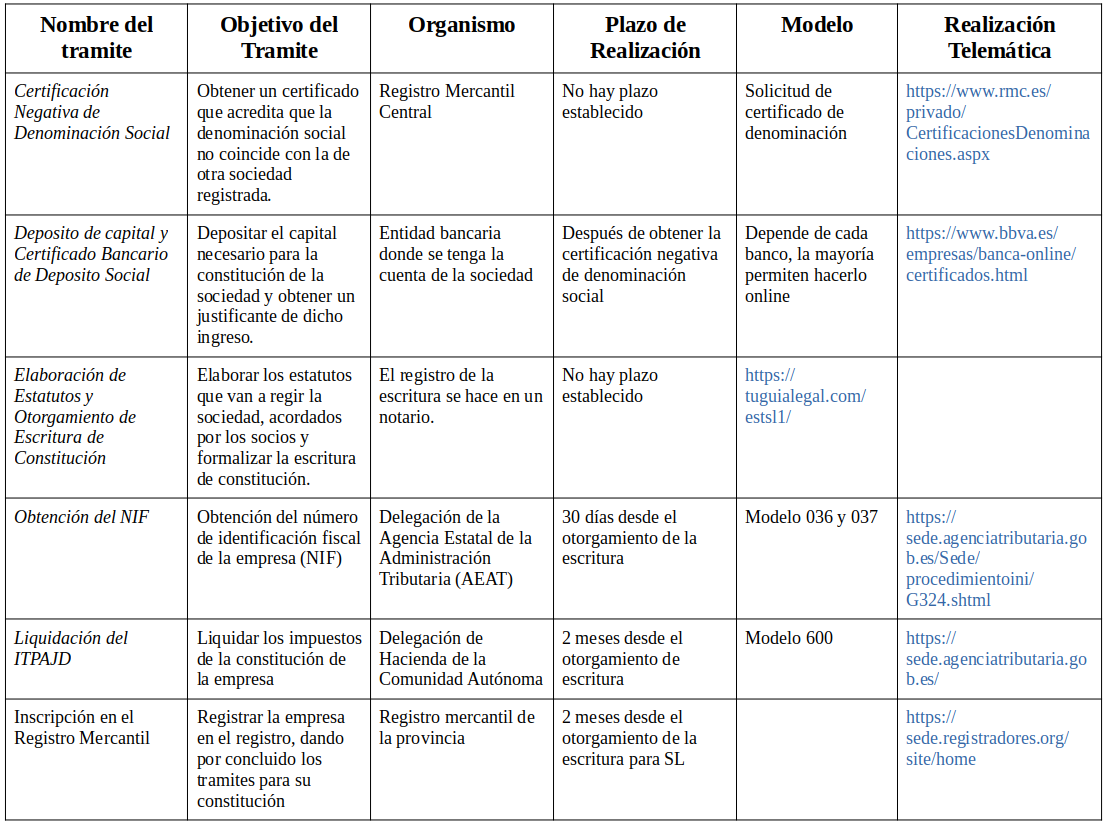
\includegraphics[scale=0.35]{tramites-constitucion.png}
\end{figure}

\subsection{Tramites de Puesta en Marcha}
Una vez hayamos constituido la empresa, deberemos comenzar con los trámites de puesta en marcha, los que se detallan a continuación exponiendo en que administración se deben llevar a cabo.

\subsubsection*{Delegación de la Agencia Estatal de la Administración Tributaria}
\begin{itemize}
    \item \textbf{Dirección}: Avenida de la Constitución, 1. 18071, Granada, Granada
    \item \textbf{Web}: \url{https://sede.agenciatributaria.gob.es/}
    \item \textbf{Teléfono}: 958 29 44 11
\end{itemize}

\begin{figure}[H]
    \centering
    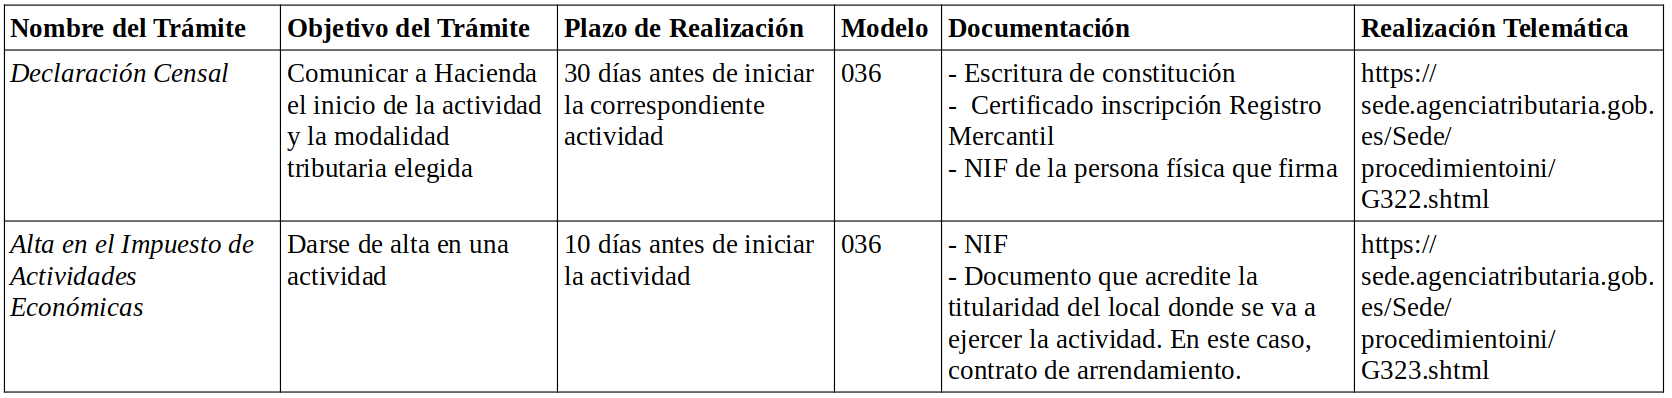
\includegraphics[scale=0.36]{tramites-AIE.png}
\end{figure}

\subsubsection*{Tesorería General de la Seguridad Social}
\begin{itemize}
    \item \textbf{Dirección}: Calle Gran Vía de Colón 23 18001 Granada (Granada)
    \item \textbf{Web}: \url{https://www.seg-social.es/wps/portal/wss/internet/Inicio}
    \item \textbf{Teléfono}: 901 50 20 50
\end{itemize}

\begin{figure}[H]
    \centering
    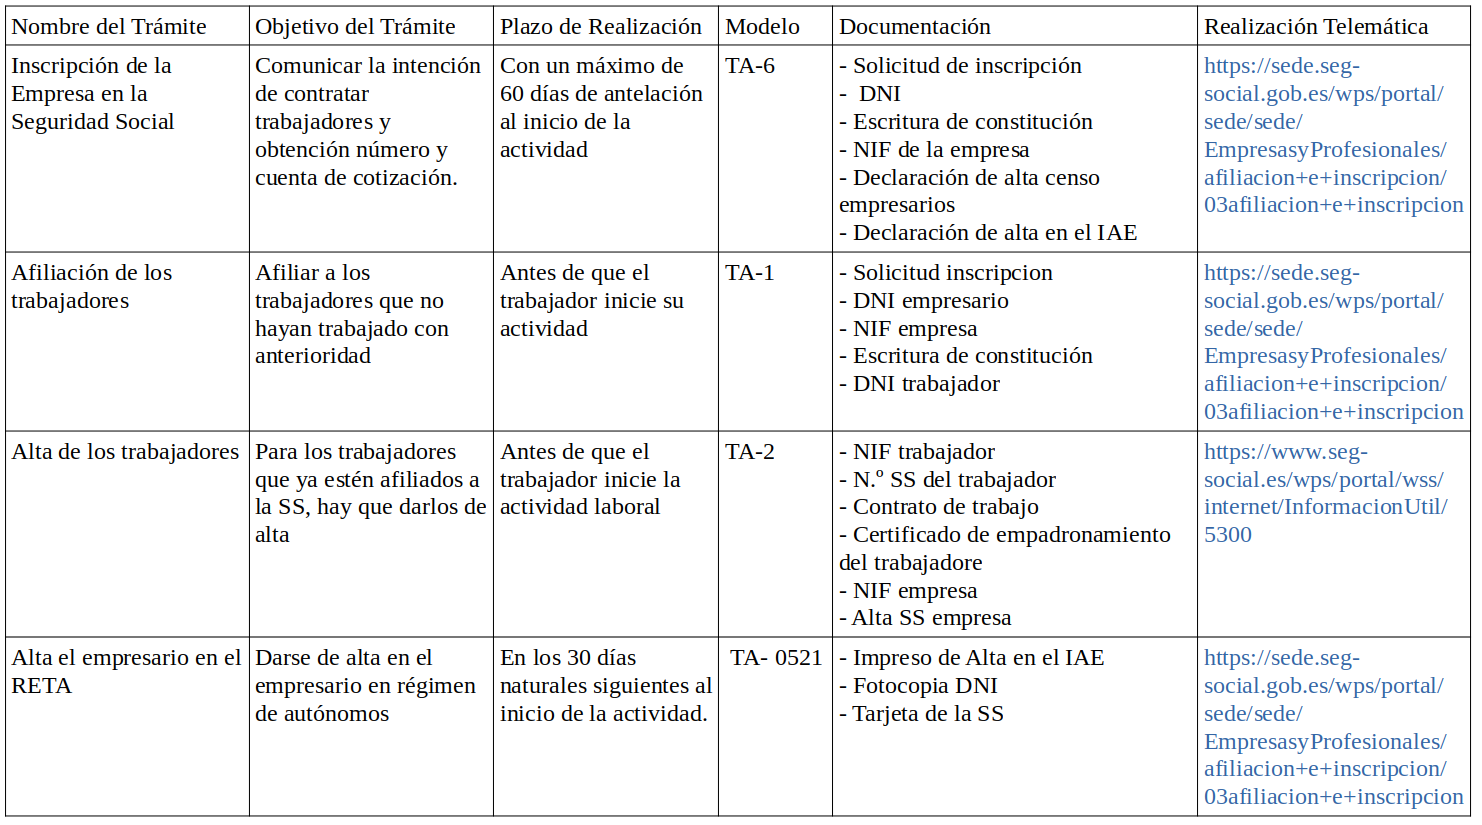
\includegraphics[scale=0.40]{tramites-SS.png}
\end{figure}

\subsubsection*{Trámites Laborales}

\begin{itemize}
    \item \textbf{En la Administración Laboral}
    \begin{itemize}
        \item \textbf{Nombre}: Delegación Territorial de Empleo, Empresa y Trabajo Autónomo en Granada
        \item \textbf{Dirección}: Calle Joaquina Eguaras 2 18013 Granada (Granada)
        \item \textbf{Web}: \url{https://www.mites.gob.es/}
        \item \textbf{Teléfono}: 958 02 73 23

        \begin{figure}[H]
            \centering
            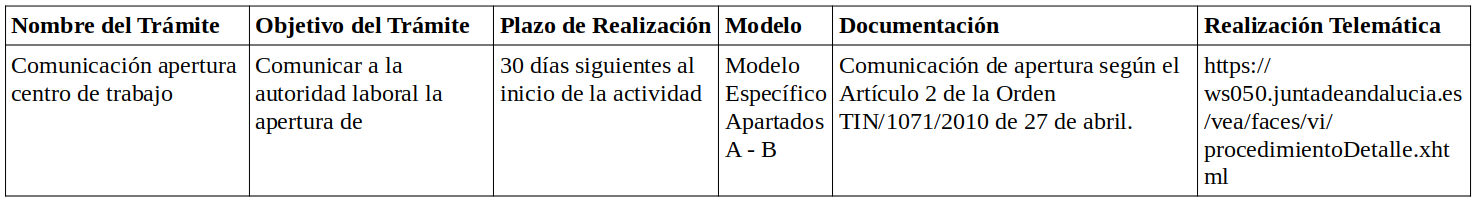
\includegraphics[scale=0.38]{tramites-laboral.png}
        \end{figure}
    \end{itemize}
    \item \textbf{En el SEPE}:
    \begin{itemize}
        \item \textbf{Dirección}:  C. Sos del Rey Católico, 3, Genil, 18006 Granada
        \item \textbf{Web}: \url{https://www.sepe.es/}
        \item \textbf{Teléfono}: 958 90 05 98

        \begin{figure}[H]
            \centering
            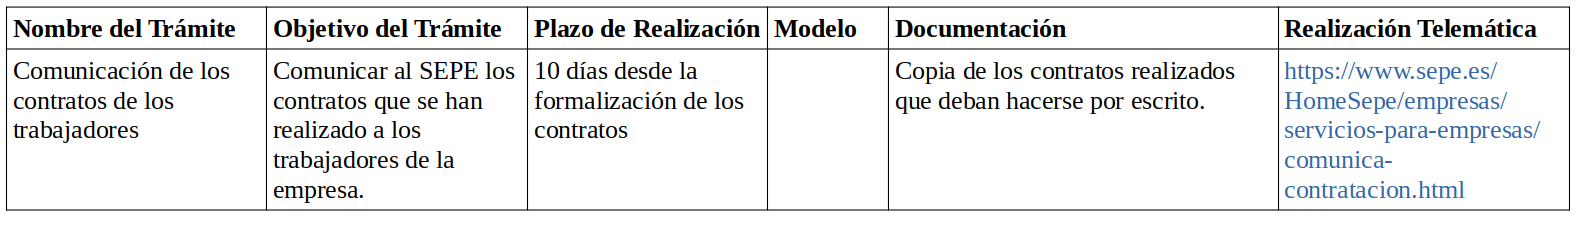
\includegraphics[scale=0.36]{tramites-SEPE.png}
        \end{figure}
    \end{itemize}
\end{itemize}

\subsubsection*{Trámites en el Ayuntamiento}
\begin{itemize}
    \item \textbf{Dirección}:  Plaza del Carmen, 18071, Granada
    \item \textbf{Web}: \url{https://www.granada.org/}
    \item \textbf{Teléfono}: 958 539 697

    \begin{figure}[H]
        \centering
        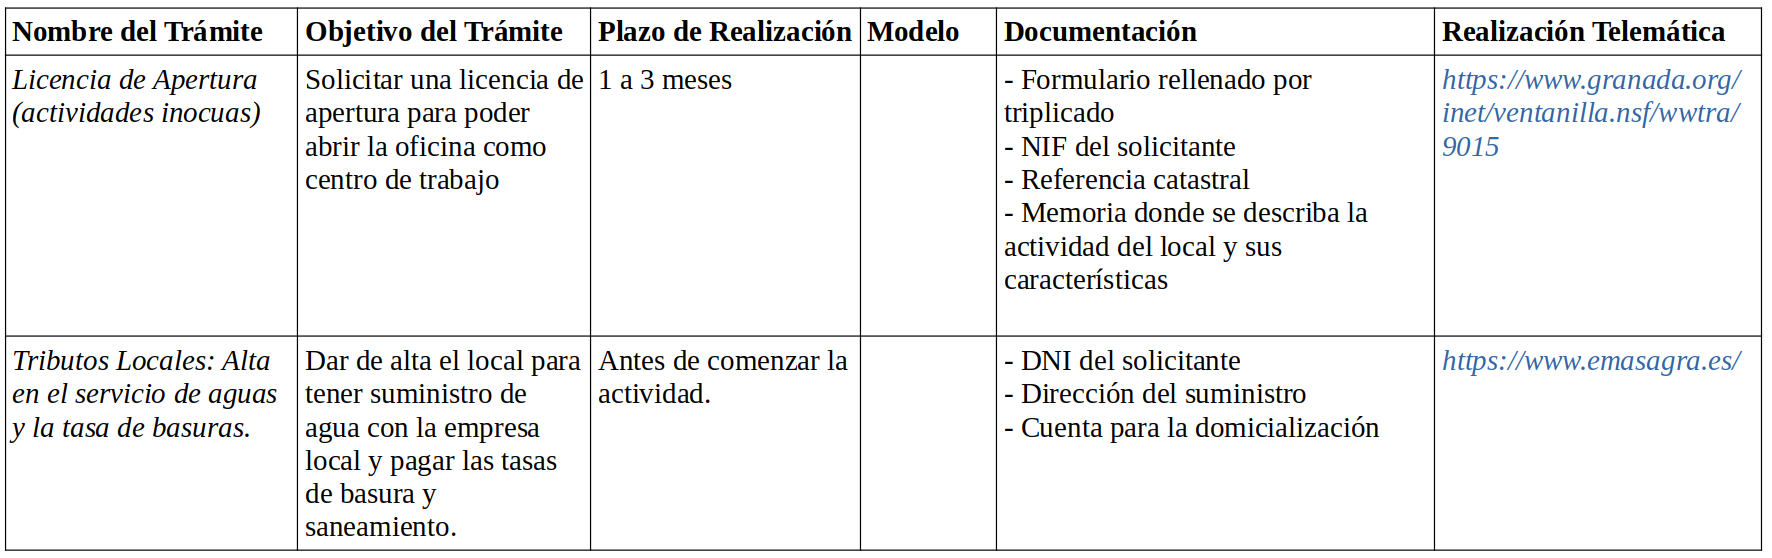
\includegraphics[scale=0.34]{tramites-ayto.png}
    \end{figure}
\end{itemize}

\subsubsection*{Otros Trámites}
Además de los tramites ya realizados, la empresa ha llevado a cabo otros trámites necesarios para su funcionamiento, los cuales se detallan
en la siguiente tabla.

\begin{figure}[H]
    \centering
    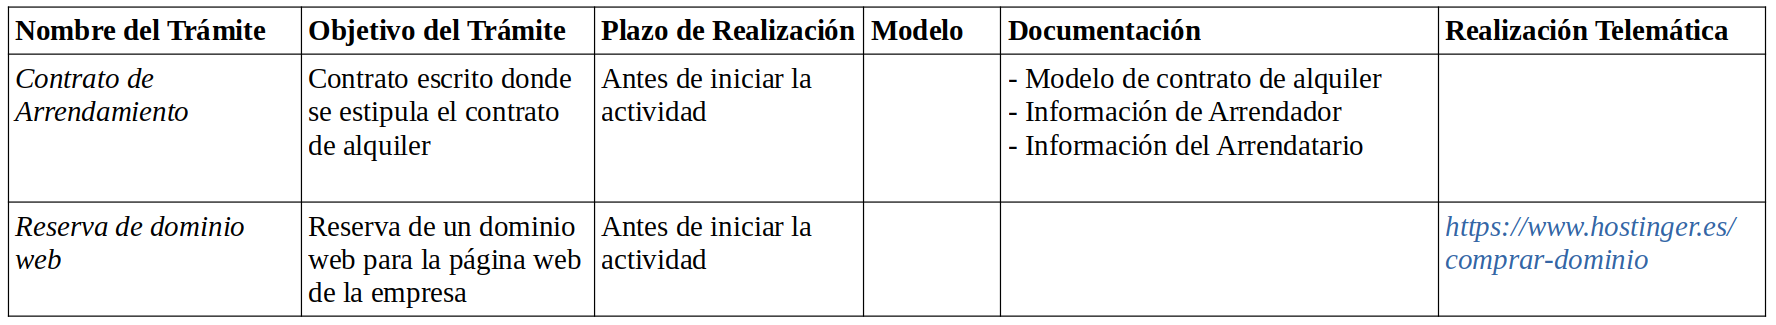
\includegraphics[scale=0.34]{tramites-otro.png}
\end{figure}


\subsection{Coste de los Trámites}
\label{sec:costetramites}
Por último, vamos a determinar cuales son los costes totales para constituir y poner en marcha la empresa, listando a continuación cada trámite y su coste.

\begin{itemize}
    \item \textbf{Coste Desglosado de Trámites}:
    \begin{itemize}
        \item Certificado Negativo de Denominación: \textbf{15,05€}
        \item Certificado Bancario Deposito Capital: \textbf{12,2€}
        \item Otorgamiento de Escritura: \textbf{50€}
        \item Obtención NIF: \textbf{Gratuito}
        \item Liquidación ITPAJD: \textbf{0€} (Creación de Sociedad)
        \item Inscripción Registro Mercantil: \textbf{150€}
        \item Declaración Censal: \textbf{0€}
        \item Alta AEAT: \textbf{0€}
        \item Inscripción Empresa SS: {0€}
        \item Afiliación de los trabajadores: \textbf{0€}
        \item Alta trabajadores SS: \textbf{0€}
        \item Alta empresario RETA: \textbf{0€}
        \item Comunicación Apertura Centro Trabajo: \textbf{0€}
        \item Comunicación Contrato Trabajadores: \textbf{0€}
        \item Licencia de Apertura: \textbf{370€}
        \item Alta Servicio de Basuras: \textbf{0€}
    \end{itemize}

    \item \textbf{Coste Total}: 597,25€
\end{itemize}

\section{Plan Económico Financiero}
En este último epígrafe, vamos a exponer el plan económico, de forma más o menos detallada, intentado realizar una previsión del primer año de funcionamiento de la empresa.

\subsection{Plan de Inversión Inicial}
En esta sección vamos a detallar la inversión inicial necesaria especificando primero los gastos e inversión que vamos a tener en agrupados según su naturaleza. Estos gastos e inversiones son los siguientes:

\begin{itemize}
    \item \textbf{Inmovilizado Material}

    Por suerte, el local que vamos a utilizar esta acondicionado como oficina y ya posee muchos de los materiales necesarios para el
    desarrollo de la actividad, pero se necesitarán ordenadores, un servidor y otros útiles de oficina, como son los siguientes:
    \begin{itemize}
        \item \textbf{Ordenadores portátiles}: ordenadores portátiles para el diseñador gráfico y los dos desarrolladores, incluido yo mismo, con un presupuesto máximo por empleado de \textbf{1500€}.
        \item \textbf{Servidor}: servidor para administrar todos los servicios del proceso de desarrollo y que además servirá de estación de trabajo para el administrador de sistema, con un presupuesto máximo de \textbf{1200€}.
        \item \textbf{4 sillas ergonómicas}: sillas para los trabajadores, ya es una de las cosas que no incluye el local, con un coste total de las 4 sillas de \textbf{500€} máximo..

        \item \textbf{Total}: 6200€
    \end{itemize}
    \item \textbf{Inmovilizado Inmaterial}:


    En este apartado se incluyen gastos como el software, fianzas, etc..
    \begin{itemize}
          \item \textbf{Software}: el software utilizado será Linux para los portátiles dedicados al desarrollo y FreeBSD para el servidor, por lo que el gasto inicial será de \textbf{0€}.
          \item \textbf{Fianza alquiler del local}: la fianza, de 2 mensualidades del local, se incluye en este apartado, suponiendo un gasto de \textbf{900€}

          \item \textbf{Total}: 900€
    \end{itemize}

    \item \textbf{Gastos de Constitución y Primer Establecimiento}
    En este punto se detallan los gastos de constitución y primer establecimiento, así como los de publicidad.
    \begin{itemize}
        \item \textbf{Constitución y Establecimiento}: Estos gastos ya están desglosados en el epígrafe \hyperref[sec:costetramites]{10.4 Costes de los Trámites}, por lo que aquí solo se detalla el coste final, que será de \textbf{597,25€}.

        \item \textbf{Publicidad}: como se ha especificado en el apartado \hyperref[sec:publi]{6.4 Política de Comunicación}, el gasto anual de asciende a 8400€, pero aquí solo tendremos en cuenta el gasto del primer mes, que será un gasto fijo durante el primer año y que se sitúa en \textbf{750€}.

        \item \textbf{Total}: 1347,25€
    \end{itemize}


    \item \textbf{Gastos de Circulante}

    En este punto se incluyen los gatos corrientes que tendrá la empresa, gastos que serán prácticamente los
    mismos cada mes, y se incluyen:

    \begin{itemize}
        \item \textbf{Alquiler del Local}: el alquiler del local, que ya incluye los gatos de agua, luz e internet, asciende a \textbf{450€}.
        \item \textbf{Provisión de fondos de la tesorería}: se ha decidido mantener una provisión de fondos en la tesorería de unos \textbf{10000€}, para poder hacer frente a pagos imprevistos.

        \item \textbf{Total}: 10450€
    \end{itemize}

    \item \textbf{Total Inversión Inicial}: 18.897,25€
\end{itemize}

\subsection{Plan de Financiación Inicial}
En este punto vamos a exponer el pan de financiación inicial, especificando los prestamos que se podrán pedir,
el capital con el que se cuenta de inicio y las ayudas que se podrán solicitar.

\begin{itemize}
    \item \textbf{Recursos propios}: inicialmente voy a poder hacer un aporte de \textbf{10000€}, dinero que tengo ahorrado en una cuenta y cuyo propósito era precisamente éste.
    \item \textbf{Préstamos}: se va a solicitar al banco \textbf{BBVA} un préstamo por valor de \textbf{10000€}. Este préstamo se pedirá haciendo uso de las \textbf{Ayudas ICO}, y se establecerá una amortización de 1 pago anual de \textbf{5000€}, durante 2 años.
\end{itemize}

\section{Previsión de la Tesorería}
En la siguiente tabla, se muestra una previsión estimada de los gatos y cobros que tendrá la empresa y que podemos ver en la siguiente tabla.

\begin{figure}[H]
    \centering
    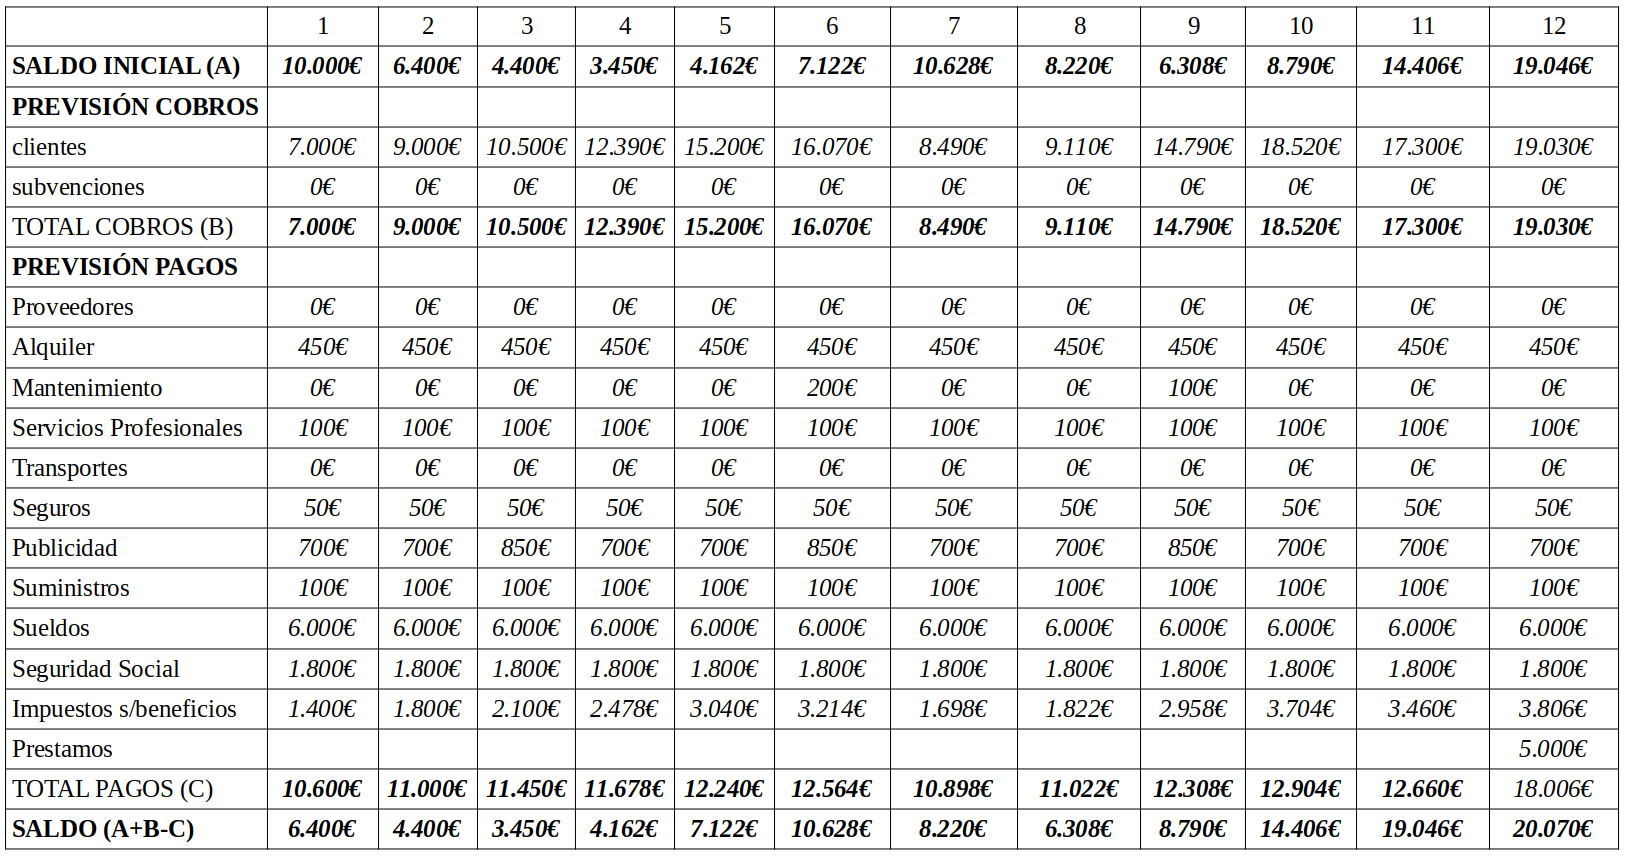
\includegraphics[scale=0.40]{prevision.png}
\end{figure}

A la hora de realizar esta previsión se han tenido en cuenta una serie de factores que vamos a mencionar a continuación:

\begin{itemize}
    \item \textbf{Numero de proyectos}: en este aspecto, el \textbf{diseñador web} puede ocuparse de entre \textbf{2 a 4 proyectos} de Wordpress al mes, dependiendo de su complejidad, teniendo en cuenta que estos proyectos tienen un precio entre \textbf{1.000€ y 5.000€} se puede esperar unos ingresos por dichos proyectos entre \textbf{4.000€ y 10.000€}, ya que si el proyecto es más complejo vale más, pero requieren más tiempo. En el caso de las \textbf{Aplicaciones Web}, su precio comienza en \textbf{5.000€}. Si no son muy complejas, se pueden llevar a cabo \textbf{2 al mes}, una para cada desarrollador, lo que supone un ingreso mínimo de \textbf{10.000€}. En el caso de aplicaciones más complejas deberán dedicarse los 2 desarrolladores y su precio será bastante más elevado. Esto hace que la estimación de ingresos mensuales se
    espera que sea entre los \textbf{15.000€ y los 28.000€}.

    \item \textbf{Servicio de Mantenimiento}: ese servicio se espera que al menos un 50\% de los clientes lo
    contrate, por lo que habría que añadir \textbf{30€} mensuales por clientes que lo ha contratado para Wordpress y \textbf{200€} mensuales para aplicaciones web. Cuantos más clientes hayan obtenido nuestros servicios más contrataciones habrá por lo que este ingreso se incrementará con el tiempo.

    \item \textbf{Meses iniciales y Verano}: se ha tenido en cuenta que los primeros meses, mientras que las estrategias de \textbf{marketing dan sus frutos}, habrá pocos proyectos, por lo que se ha estimado a la baja. En los meses subsiguientes la facturación aumentará. Además, cuantos más clientes hayan pasado por la empresa, también aumentará la captación de clientes con el boca a boca.  Además, en verano hay muchas empresas que cierran y se van de vacaciones, por lo que los meses de \textbf{Julio y Agosto} se han estimado a la baja.

    \item \textbf{Meses de Septiembre a Diciembre}: al contrario que en el punto anterior durante estos meses hay mucha actividad empresaria, además, se comienzan a preparar las campañas de navidad, por lo que habrá un incremento sustancial en la facturación.
\end{itemize}

\section{Cuenta de Perdidas y Ganancias Previsional}
Por último, vamos a mostrar una tabla con el balance anual de perdidas y ganancias que estimamos podrá tener la empresa, el cual podemos ver en la siguiente tabla.

\begin{figure}[H]
    \centering
    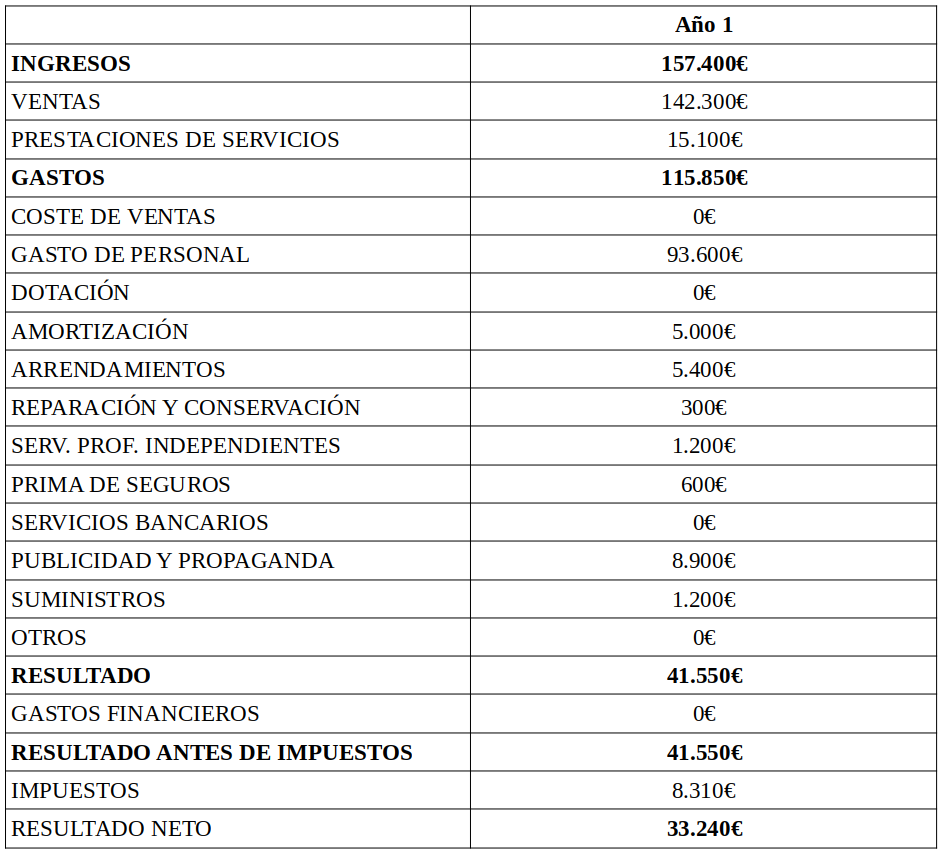
\includegraphics[scale=0.45]{beneficio.png}
\end{figure}

Como vemos, el beneficio neto es de \textbf{10.070€}, en comparación con la inversión inicial total de \textbf{18.897,25€}, lo que podría hacer pensar que el negocio no es viable. Esto también se debe a que solo se ha realizado la previsión del primer año y los primeros meses a este tipo de empresas les cuesta arrancar,  ya que depende en parte de generar una buena base de clientes, lo que lleva unos meses.

Con los datos de los últimos meses del año, cabe esperar que en el 2º año se haya recuperado la inversión y con un ratio de beneficio bastante superior al que podríamos esperar en un banco u otro tipo de inversión. Esto se podría ver mejor si se hubiera realizado la previsión del segundo año también.

\section{Nos Valoramos}
La verdad es que algunas cosas se podrían haber mejorado, quizá la previsión y la configuración de la plantilla de trabajadores, ya que no tengo muy claro que se necesite un administrador de sistemas para el tamaño de la empresa, lo que sería un ahorro sustancial. Si voy con tiempo de sobra para la siguiente práctica cambiaré eso.

Al margen de eso lo he hecho bien, así que me pondría un 7.5 u 8 de nota.

% Bibliography

%\newpage
%\bibliography{citas}
%\bibliographystyle{unsrt}

\end{document}